% Do not modify the template. Enter your solution in the indicated locations only.
\documentclass[answers,a4paper,11pt]{exam}
\usepackage[top=2cm,bottom=2.5cm,left=1cm,right=1.5cm,a4paper]{geometry}
\usepackage{graphicx}
\usepackage{amsmath}
\usepackage{amssymb}
\usepackage[shortlabels]{enumitem}

\pagestyle{headandfoot}
\lhead{Deadline: Week 6, Tuesday 23:59.} % Week number
%\chead{At-home assignment}
\rhead{T-304-CACS}
\cfoot{Calculus for Computer Science}
\rfoot{Page \thepage{} of \numpages}

\begin{document}

\noindent
\textbf{Name: Jóhann Berentsson} % WRITE YOUR NAME HERE

\vspace{0.5em}
\noindent
\textbf{Kennitala: 050188-2489} % WRITE YOUR KENNITALA HERE

\vspace{0.5em}
\noindent
Explain your solution concisely but clearly. Include all derivation steps. Make sure a fellow student would be able to understand what you mean.

\begin{questions}

% PROBLEM 1
\question
Use L'H\^opital's rule as many times as necessary to find the following limit. State \emph{why} you can use L'H\^opital's rule. (What condition needs to be satisfied?)
\[
L = \lim_{x\to 0} \frac{(x+1) e^{-x} - 1}{\sin^2 x}
\]
    
\begin{tabular}{| l | l |}
    \hline
    \begin{tabular}{l}
        Volume of a cylinder: $V=h \pi r^2$
    \end{tabular}
    &
    \begin{tabular}{l}
        Surface area of a cylinder: $A=(2 \pi r^2) + (2 \pi r h)$
    \end{tabular} \\
    \hline
\end{tabular}

\begin{tabular}{| l | l | l | l |}
    \hline
    \begin{tabular}{l}
        \textbf{1. Isolate h} \\
        \textbf{for surface.} \\
        $A=(2 \pi r^2) + (2 \pi r h)$ \\\\
        $2 \pi r^2 = A - 2 \pi r^2$ \\\\
        $h = \frac{A - 2 \pi r^2}{2 \pi r}$ \\\\\\\\\\\\\\\\
    \end{tabular}
&
    \begin{tabular}{l}
        \textbf{2. Insert the} \\
        \textbf{volume formula.} \\
        $h = \frac{A - 2 \pi r^2}{2 pi r}$ \\\\
        $V=h \pi r^2$ \\\\
        $V= (\frac{A - 2 \pi r^2}{2 \pi r}) \pi r^2$ \\\\
        $V = \frac{(A \pi r^2) - (2 \pi^2 r^4)}{2 \pi r}$ \\\\
        $V = \frac{A \pi r^2}{2 \pi r} - \frac{2 \pi^2 r^4}{2 \pi r}$ \\\\
        $V = \frac{A r}{2} - \pi r^3$ \\\\
    \end{tabular}
&
    \begin{tabular}{l}
        \textbf{3. Find derivative.}\\
        $V(r) = \frac{A r}{2} - \pi r^3$ \\\\
        $V'(r) = \frac{A r}{2} - 3 \pi r^2$ \\\\
        $V'(r) = \frac{A}{2} - 3 \pi r^2$ \\\\\\\\\\\\\\\
    \end{tabular}
&
    \begin{tabular}{l}
        \textbf{4. Critical point.}\\
        $V'(r) = \frac{A}{2} - 3 \pi r^2 = 0$ \\\\
        $3 \pi r^2 = \frac{A}{2}$ \\\\
        $r^2 = \frac{A}{(3 \times 2) \pi}$ \\\\
        $r = \sqrt{\frac{A}{(3 \times 2) \pi}}$ \\\\
        $r = \sqrt{\frac{A}{6 \pi}}$ \\\\\
    \end{tabular}
    \\
\hline
\end{tabular}

\begin{tabular}{| l  l | l |}
    \hline
    \textbf{5. Find h for volume} && \textbf{6. Volume} \\
    \begin{tabular}{l}
        $r = \sqrt{\frac{A}{6 \pi}}$ \\\\\
        $h = \frac{A - 2 \pi r^2}{2 \pi r}$ \\\\
        $h = \frac{A - 2 \pi (\sqrt{\frac{A}{6 \pi}})^2}{2 \pi (\sqrt{\frac{A}{6 \pi})}}$ \\\\
        $h = \frac{A - 2 \pi (\frac{A}{6 \pi})}{2 \pi (\sqrt{\frac{A}{6 \pi})}}$ \\\\
        $h = \frac{A - \frac{2 \pi A}{6 \pi}}{2 \pi \sqrt{\frac{2 \pi A}{6 \pi}}}$ \\\\
        $h = \frac{A - \frac{A}{3}}{2 \pi \sqrt{\frac{2 \pi A}{6 \pi}}}$ \\\\
        $h = \frac{\frac{3A}{3} - \frac{A}{3}}{2 \pi \sqrt{\frac{2 \pi A}{6 \pi}}}$ \\\\
        $h = \frac{\frac{3A - A}{3}}{2 \pi \sqrt{\frac{2 \pi A}{6 \pi}}}$ \\\\
    \end{tabular}{}
    &
    \begin{tabular}{l}
        $h = \frac{\frac{2A}{3}}{2 \pi \sqrt{\frac{2 \pi A}{6 \pi}}}$ \\\\
        $h = \frac{\frac{2A}{3}}{2 \pi \sqrt{\frac{2 \pi A}{6 \pi}}}$ \\\\
        $h = \frac{2A}{3} \times \frac{1}{\sqrt{\frac{2 \pi A}{6 \pi}}}$ \\\\
        $h = \frac{2A}{3} \times \frac{1}{2 \pi \sqrt{\frac{A}{6 \pi}}}$ \\\\
        $h = \frac{2A}{3} \times \frac{1}{\frac{2 \pi \sqrt{A}}{\sqrt{6 \pi}}}$ \\\\
        $h = \frac{2A}{3} \times \frac{\sqrt{6 \pi}}{2 \pi \sqrt{A}}$ \\\\
        $h = \frac{(2A) (\sqrt{6 \pi})}{(3)(2 \pi \sqrt{A})}$ \\\\
        $h = \frac{2A \sqrt{6\pi}}{6 \pi \sqrt{A}} = \frac{\sqrt{12 \pi A}}{\sqrt{6 \pi A}}$ \\\\
        $h = \frac{\sqrt{6\pi A}}{3 \pi}$ \\\\
    \end{tabular}{}
    &
    \begin{tabular}{l}
        $V = h \times \pi \times r^2$\\
        $V = \frac{\sqrt{6\pi A}}{3 \pi} \times \pi \times (\sqrt{\frac{A}{6 \pi}})^2$\\\\
        $V = \frac{\sqrt{6\pi A}}{3 \pi} \times \pi \times \frac{A}{6 \pi}$\\\\
        $V = \frac{\sqrt{6 \pi A} \times \pi \times A}{3\pi \times 1 \times 6\pi}$ \\\\\
        $V = \frac{\sqrt{6 \pi A} \times A}{3\pi \times 6\pi}$ \\\\\
        $\boxed{V = \frac{A\sqrt{6 \pi A}}{18 \pi^2}}$ \\\\\\\\\\\\\\\\\\\\\\
    \end{tabular}{}
    \\
\hline
\end{tabular}

    
\newpage

% PROBLEM 2
\question
Consider the function
\[
f(x) = \frac{x^2+2 x+1}{x^2+3 x+3}
\]
\begin{enumerate}
\item Make a sketch of the function and observe where it reaches its smallest and largest value. Use GeoGebra or any other tool for plotting.
\item State what the value of $f'(x)$ is at the points $x$ where $f(x)$ reaches its smallest and largest value (``bottom of the valley'', ``peak of the mountain'').
\item Find a formula for $f'(x)$. Simplify it fully.
\item Solve the equation $f'(x) = 0$. This gives the location of the maximum and minimum.
\end{enumerate}

\begin{solutionbox}{\stretch{-1}}\newline
\section*{1. Plot of $f(xrcfgvfr) = \frac{x^2 + 2x + 1}{x^2 + 3x +3}$}
\[
    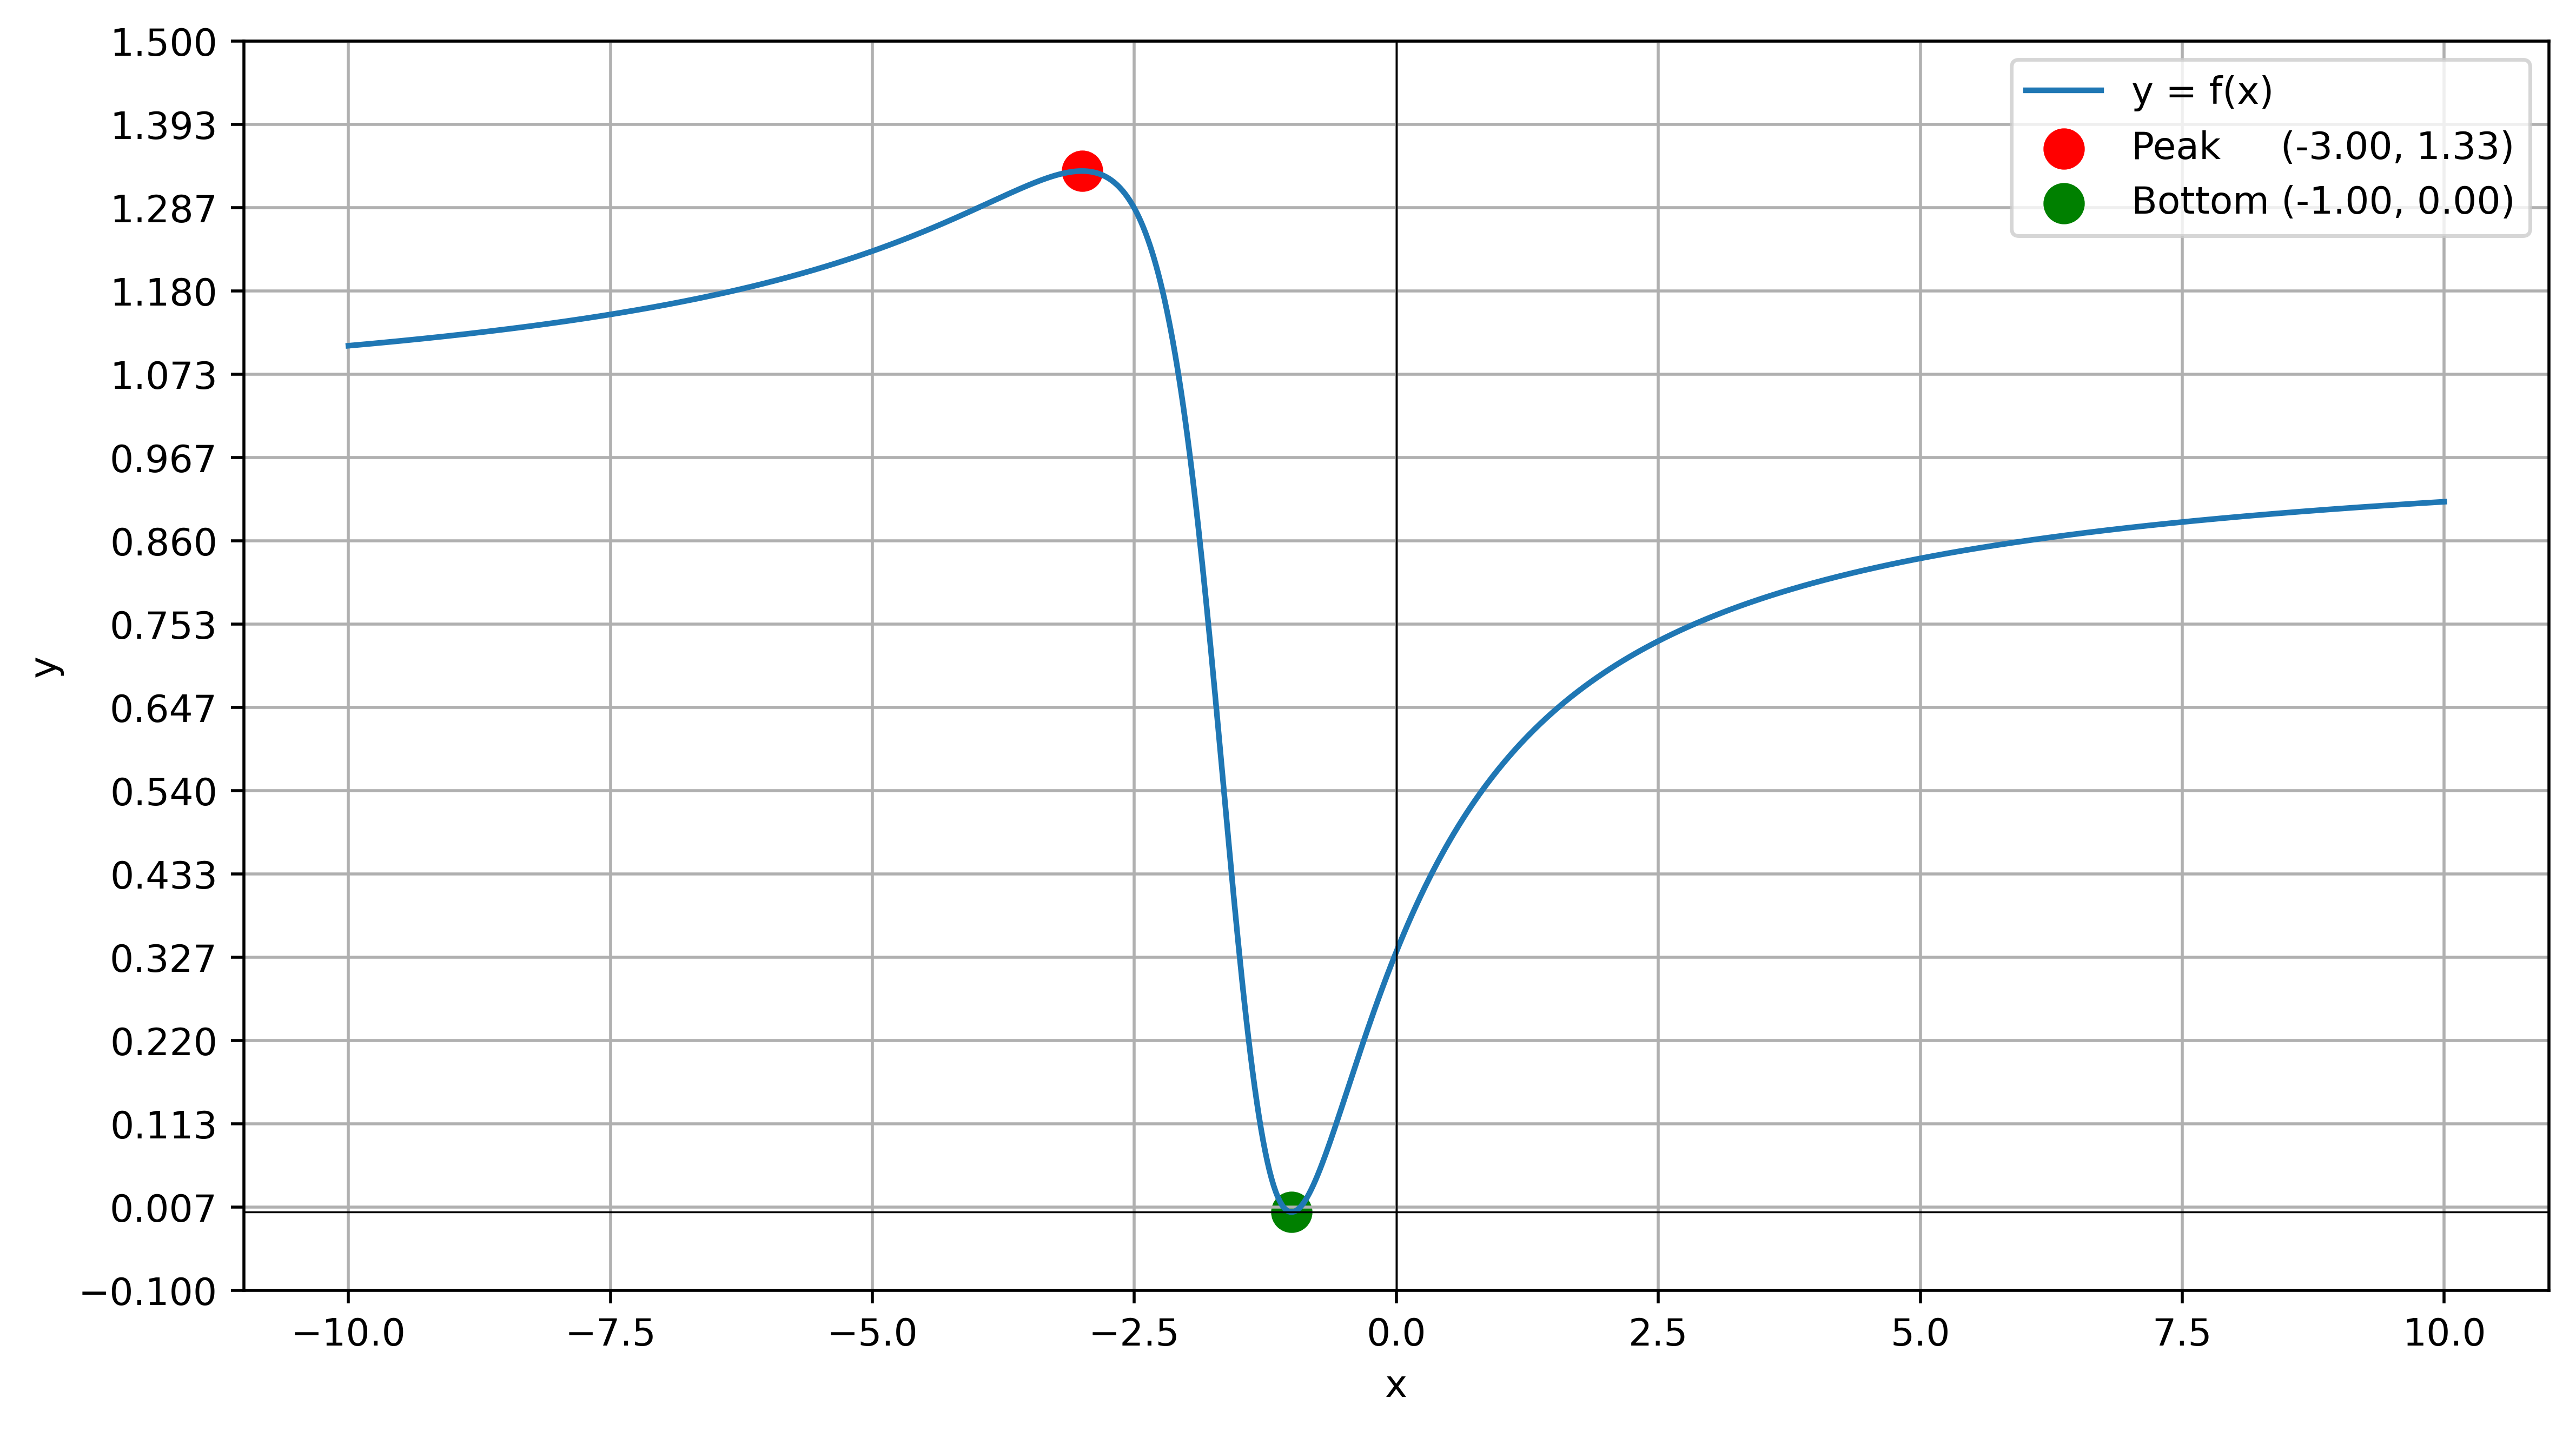
\includegraphics[scale=0.7]{plot.png}
\]

\end{solutionbox}
\newpage
\begin{solutionbox}{\stretch{-1}}\newline

\section*{2.}
\[
    f(x) = \frac{g(x)}{h(x)}= \frac{x^2 + 2x + 1}{x^2 + 3x + 3}
\]

\[
    f'(x) = \frac{(f'(x)g(x))+(f(x)g'(x))}{(g(x))^2}
\]

\[
    = \frac{(2x+2)(x^2 + 3x + 3) - (x^2 + 2x + 1)(2x+3)}{(x^2 + 3x + 3)^2}
\]

\[
    = \frac{(2x^3 + 6x^2 + 6x + 2x^2 + 6x + 6)-(2x^3 + 3x^2 + 4x^2 + 6x + 2x + 7)}{(x^4+3x^3 + 3x^2 + 3x^3 + 9x^2 + 9x + 3x^2 + 9x + 9)}
\]

\[
    = \frac{(2x^3 + 8x^2 + 12x + 6 - 2x^3 - 7x^2 - 8x - 3)}{(x^4 + 6x^3 + 15x^3 + 18x + 9)}
\]

\[
    = \frac{x^2 - 4x + 3}{x^4 + 6x^3 + 15x^2 + 18x + 9}
\]

\[
    = \frac{(x+1)(x+3)}{(x^2 + 3x + 3)^2}
\]

\subsection*{Critical Points:}

\[x = -1\]

\[x = -3\]

\section*{3.}
The formula for $f'(x)$ is:
\[
 f'(x)= \frac{(x+1)(x+3)}{(x^2 + 3x + 3)^2}
\]

See section 2. for full proof.
\end{solutionbox}
\newpage
\begin{solutionbox}{\stretch{-1}}\newline


\section*{4.}

% TODO: DO THIS AND DO THAT!

\end{solutionbox}


\end{questions}        
\end{document}
